%%%%%%%%%%%%
% Preamble %
%%%%%%%%%%%%
% set document type, section numbering, and biblography style
\documentclass[twoside, 12pt]{article}
\usepackage{fullpage, graphicx, mathtools, gensymb, mhchem, siunitx, xr, xcolor, float}
\usepackage[english]{babel}
\usepackage[labelfont=bf]{caption} 
\usepackage[super,sort&compress,comma,round]{natbib}

% set fonts
\renewcommand*\familydefault{\sfdefault}
%\usepackage{sansmathfonts}

% highlight Chris's changes and comments
\newcommand{\car}[1]{\color{blue}#1\color{black}}
\newcommand{\comment}[1]{\color{red}#1\color{black}}

% other new commands
\newcommand{\velst}{$v_\mathrm{elst}$}
\newcommand{\rb}{$\rho_\mathrm{B}$}
% set the title material
\title{\vspace{-1em}\textbf{Excitation Shift of Retinal in channelrhodopsin}}
\author{\normalsize Nico and Cris}
\date{\normalsize \today}

%%%%%%%%%%%%%
% Main Text %
%%%%%%%%%%%%%
\begin{document}
\maketitle
%\tableofcontents
%%%%%%%%%%%%%%%%
% Introduction %
%%%%%%%%%%%%%%%%
\section{Overview}

The goal of this project is to assess the approximation:
\begin{equation}
\langle \hat{O}[\rho]\rangle \approx \hat{O}[\langle \rho \rangle]
\end{equation}
for the description of an average environment, applied to the first excitation ($\pi\to\pi^*$) of the embedded retinal in the Channelrhodopsin protein. See figure \ref{fig:mos} for the molecular orbitals involved in this excitation.\\
However, a particular challenge of this project is the fact that the solute, in this case retinal, is not rigid. In fact, the structure change of the retinal along the trajectory has a considerably important effect on the first excitation energy, generating shifts as large as approx. 0.7 eV, even larger than the environment effect, which is around 0.3-0.4eV \cite{Suliman2020}.

%%%%%%%%%%%%%%%%%%%%%%%%%%%%%%%%%
% Orbitals
\begin{figure}[H]
\centering
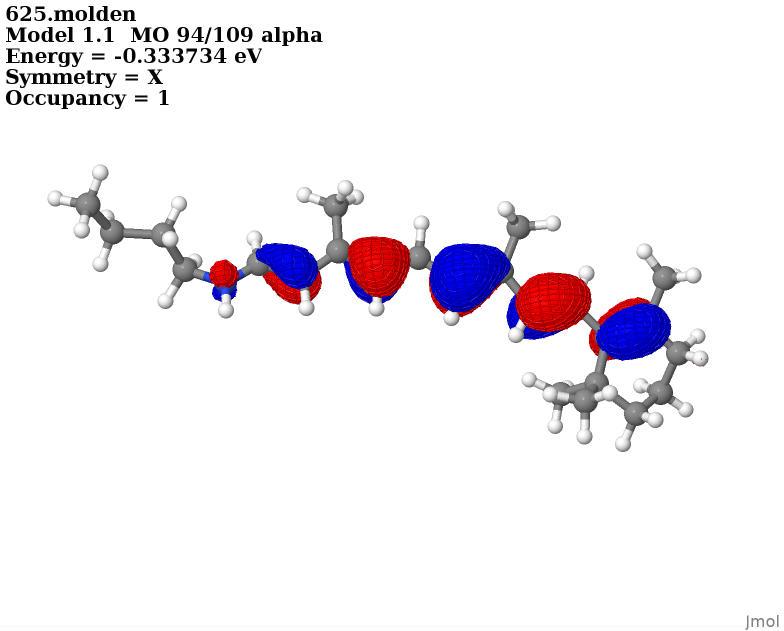
\includegraphics[width=8cm]{./figures/625_94.jpg}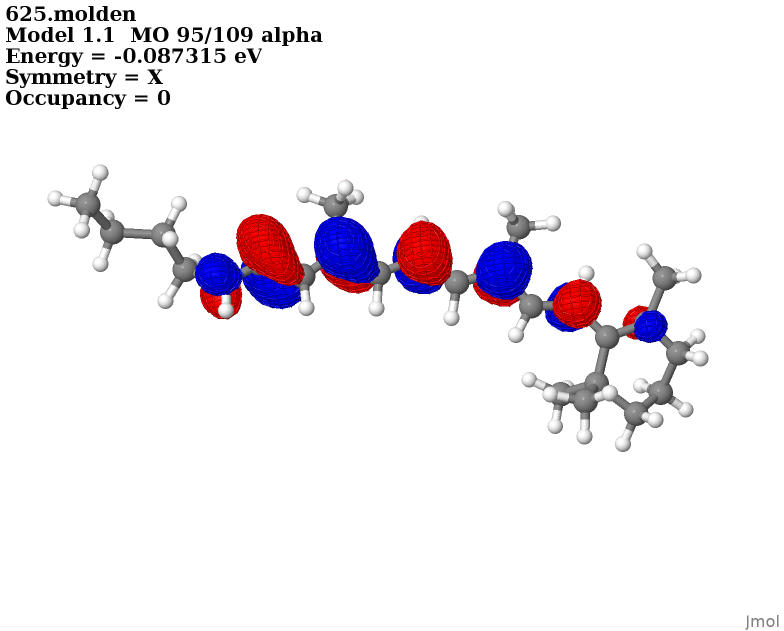
\includegraphics[width=8cm]{./figures/625_95.jpg}
\caption{Frontier molecular orbitals of retinal, HOMO the top, and LUMO at the bottom, where the excitation happens. The isosurface cutoff used was 0.03 a.u.} 
\label{fig:mos}
\end{figure}
%%%%%%%%%%%%%%%%%%%%%%%%%%%%%%%%%


%%%%%%%%%%%
% Results %
%%%%%%%%%%%
\section{Initial Results}

%%%%%%%%%%%%%%%%%%%%%
% Isolated retinal  %
%%%%%%%%%%%%%%%%%%%%%
\subsection{Spectrum of retinal}
\label{sec:init_results}
A MD trajectory of 750 frames, where all the atoms around the retinal in a radius of 12 \AA. where taken into account in different ways: the atoms within 5 \AA.  are computed as superposed electron densities, and the rest as point-charges.
The first excitation energy of the isolated retinal and the embedded retinal were computed with ADC(1)/cc-pvdz.
The corresponding spectrum is shown in \ref{fig:spec}. The averages are at 3.044 eV, for the embedded retinal at 3.418 eV, giving a shift of 0.374 eV.
As shown in figure \ref{fig:spec}, the peaks lay in 3.04 eV for the iso and 3.43 eV for embedded system. Using pointier Gaussian function (multiplying the exponential to 25.0) we obtain figure \ref{fig:spec_pt} the maximum are at 3.01 eV and 3.40 respectively [shift of 0.39 eV].


%%%%%%%%%%%%%%%%%%%%%%%%%%%%%%%%%
% Spectrum
\begin{figure}[H]
\centering
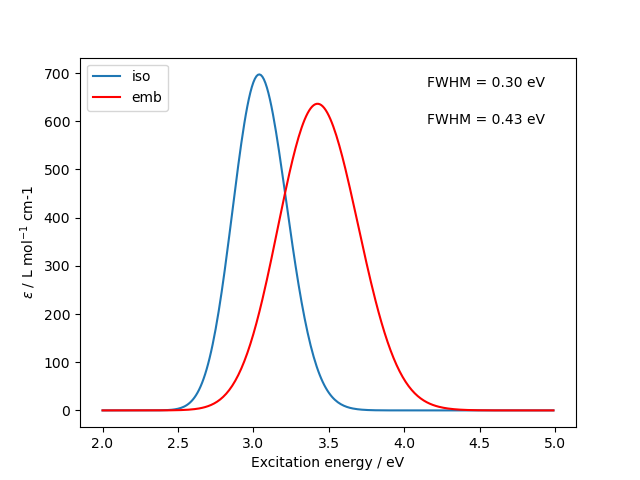
\includegraphics[width=10cm]{./figures/both_spectrum.png}
\caption{Spectrum of retinal from 750 frames MD trajectory.} 
\label{fig:spec}
\end{figure}
%%%%%%%%%%%%%%%%%%%%%%%%%%%%%%%%%

%%%%%%%%%%%%%%%%%%%%%%%%%%%%%%%%%
% Spectrum
\begin{figure}[H]
\centering
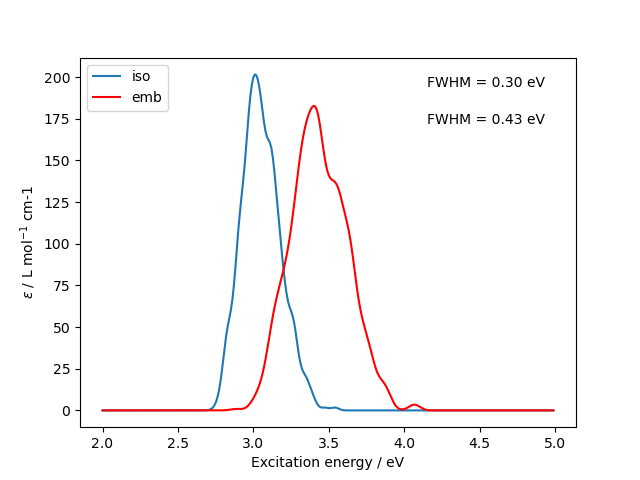
\includegraphics[width=10cm]{./figures/both_spectrum_pointy.png}
\caption{Spectrum of retinal from 750 frames MD trajectory.} 
\label{fig:spec_pt}
\end{figure}
%%%%%%%%%%%%%%%%%%%%%%%%%%%%%%%%%

When plotting:
\begin{equation}
a(x) = \sum_i \frac{f_i}{\sum_j f_j} \exp\left(-\frac{1}{2}\,c_{exp}\left(\frac{x - \epsilon_i}{\sigma}\right)^{2}\right) 
\label{eq:lineshape}
\end{equation}
where ${f_i}$ are the oscillator strengths, $\epsilon_i$ are excitation energies in eV, and $c_{exp}$ is a constant that determines the sharpness of the Gaussian functions used, the peaks seem to appear at 3.17 eV and 3.56 eV for the isolated and the embedded retinal respectively. The solvatochromic shift is 0.39 eV.


%%%%%%%%%%%%%%%%%%%%%%%%%%%%%%%%%
% Spectrum
\begin{figure}[H]
\centering
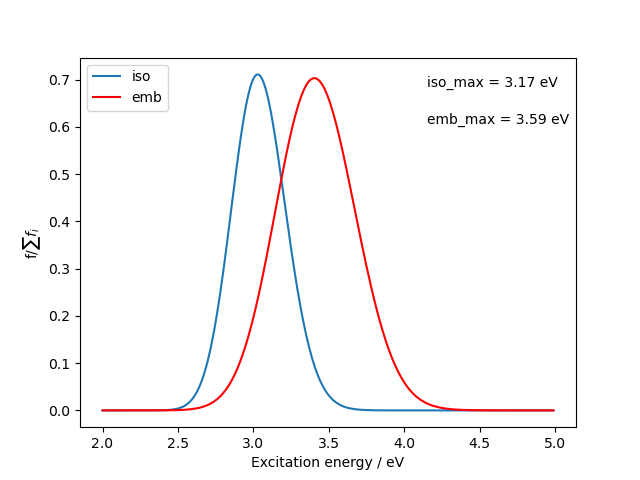
\includegraphics[width=9cm]{./figures/both_lineshape_broad.png}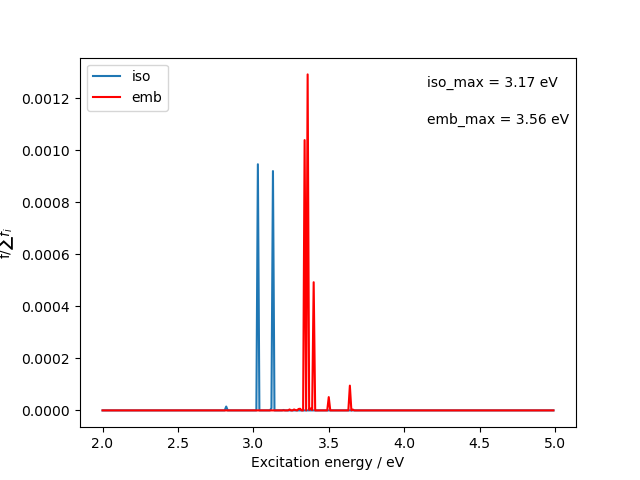
\includegraphics[width=9cm]{./figures/both_lineshape_sharp.png}
\caption{Lineshapes from 750 frames MD trajectory, following equation \ref{eq:lineshape}. Top: $c_{exp}$=1.0, bottom $c_{exp}$=$10^{8}$. } 
\label{fig:lineshape}
\end{figure}
%%%%%%%%%%%%%%%%%%%%%%%%%%%%%%%%%



\subsection{Average of Retinal}
Using the multiple methods used by Nico we generated 

%%%%%%%%%%%%%%%%%%%%%%%%%%%%
% Excitation energy table 
\begin{table}[h]
\footnotesize
\centering
\caption{Bond alternation averages in eV.}
\label{tab:ex_ret_avrg}
\begin{tabular}{lc}
& \textbf{$\varepsilon_\mathrm{gas}$ / eV} \\ 
\textbf{mb-mb} & 3.141 \\ 
\textbf{mb-pf} & 3.060 \\ 
\textbf{none-mb} & 3.132 \\ 
\textbf{none-pf} & 2.812 \\ 
\textbf{pf-mb} & 2.717 \\ 
\textbf{pf-pf} & 3.152\\ 
\textbf{Avg. 750} &  3.044 \\ 
\textbf{Std. Dev. 750} &  0.126\\ 
\end{tabular}
\end{table}
%%%%%%%%%%%%%%%%%%%%%%%%%%


\subsection{Bond-length-alternation bins}
The bond-length-alternation has been shown to be more important to the excitation energy than the environment. The bins containing frames which correspond to the 6 important basins were given by Suli. These frames were used to evaluate the average excitation energies for both the isolated and embedded retinal. The results are compared to the total-750-frames average values in table \ref{tab:ex_bins}.

We need to check if this are correct for the final trajectory shared because the averages don't seem so different.

%%%%%%%%%%%%%%%%%%%%%%%%%%%%
% Excitation energy table 
\begin{table}[h]
\footnotesize
\centering
\caption{Bond alternation averages in eV.}
\label{tab:ex_bins}
\begin{tabular}{cccc}
& \textbf{$\langle \varepsilon_\mathrm{gas} \rangle$ / eV} & \textbf{$\langle \varepsilon_\mathrm{emb} \rangle$ / eV} & \textbf{$\delta \varepsilon$ / eV}  \\ 
\textbf{Bin 1} & 2.989 & 3.286 & 0.297\\ 
\textbf{Bin 2} & 3.043 & 3.415 & 0.372\\ 
\textbf{Bin 3} & 3.044 & 3.418 & 0.374\\ 
\textbf{Bin 4} & 3.040 & 3.412 & 0.372\\ 
\textbf{Bin 5} & 3.055 & 3.438 & 0.383\\ 
\textbf{Bin 6} & 3.136 & 3.486 & 0.350\\ 
\textbf{Avg. 750} &  3.044 & 3.418 & 0.374\\ 
\textbf{Std. Dev. 750} &  0.126 & 0.183 &\\ 
\end{tabular}
\end{table}
%%%%%%%%%%%%%%%%%%%%%%%%%%


%%%%%%%%%%%%%%%%
% Bibliography %
%%%%%%%%%%%%%%%%
\clearpage
%\bibliography{references}
\bibliographystyle{achemso}

\end{document}





































